\chapter{SYSTEM IMPLEMENTATION}

With all the system design and system analysis completed in the previous semester, we now embark on the implementation phase of our project. This chapter details the process of bringing our design to life, outlining the key features of our system and the methodologies employed to implement them. Through careful planning and execution, we aim to translate our theoretical framework into a functional and efficient system. Below are some of the critical features of our system and the approaches we used to implement them.


\section{Caching Mechanism}

To reduce the amount of time it takes to access frequently accessed data
and increase the general system performance, we will apply caching data
in our system. The applied caching strategy is called \emph{aside
    caching} \emph{(Figure 5.1).} The detailed caching process is as follows:

- Step 1: The application will check whether the cache has the data it
needs or not.

- Step 2: If the cache has the data the application needs, the process
will end. If the cache has no data, we will go to the next step.

- Step 3: When the cache does not contain the data that the application
needs, the application will go to the database to get the data

- Step 4: The application will save the data retrieved from the database
to the cache, then it will continue its work.

\begin{figure}[H]
    \centering
    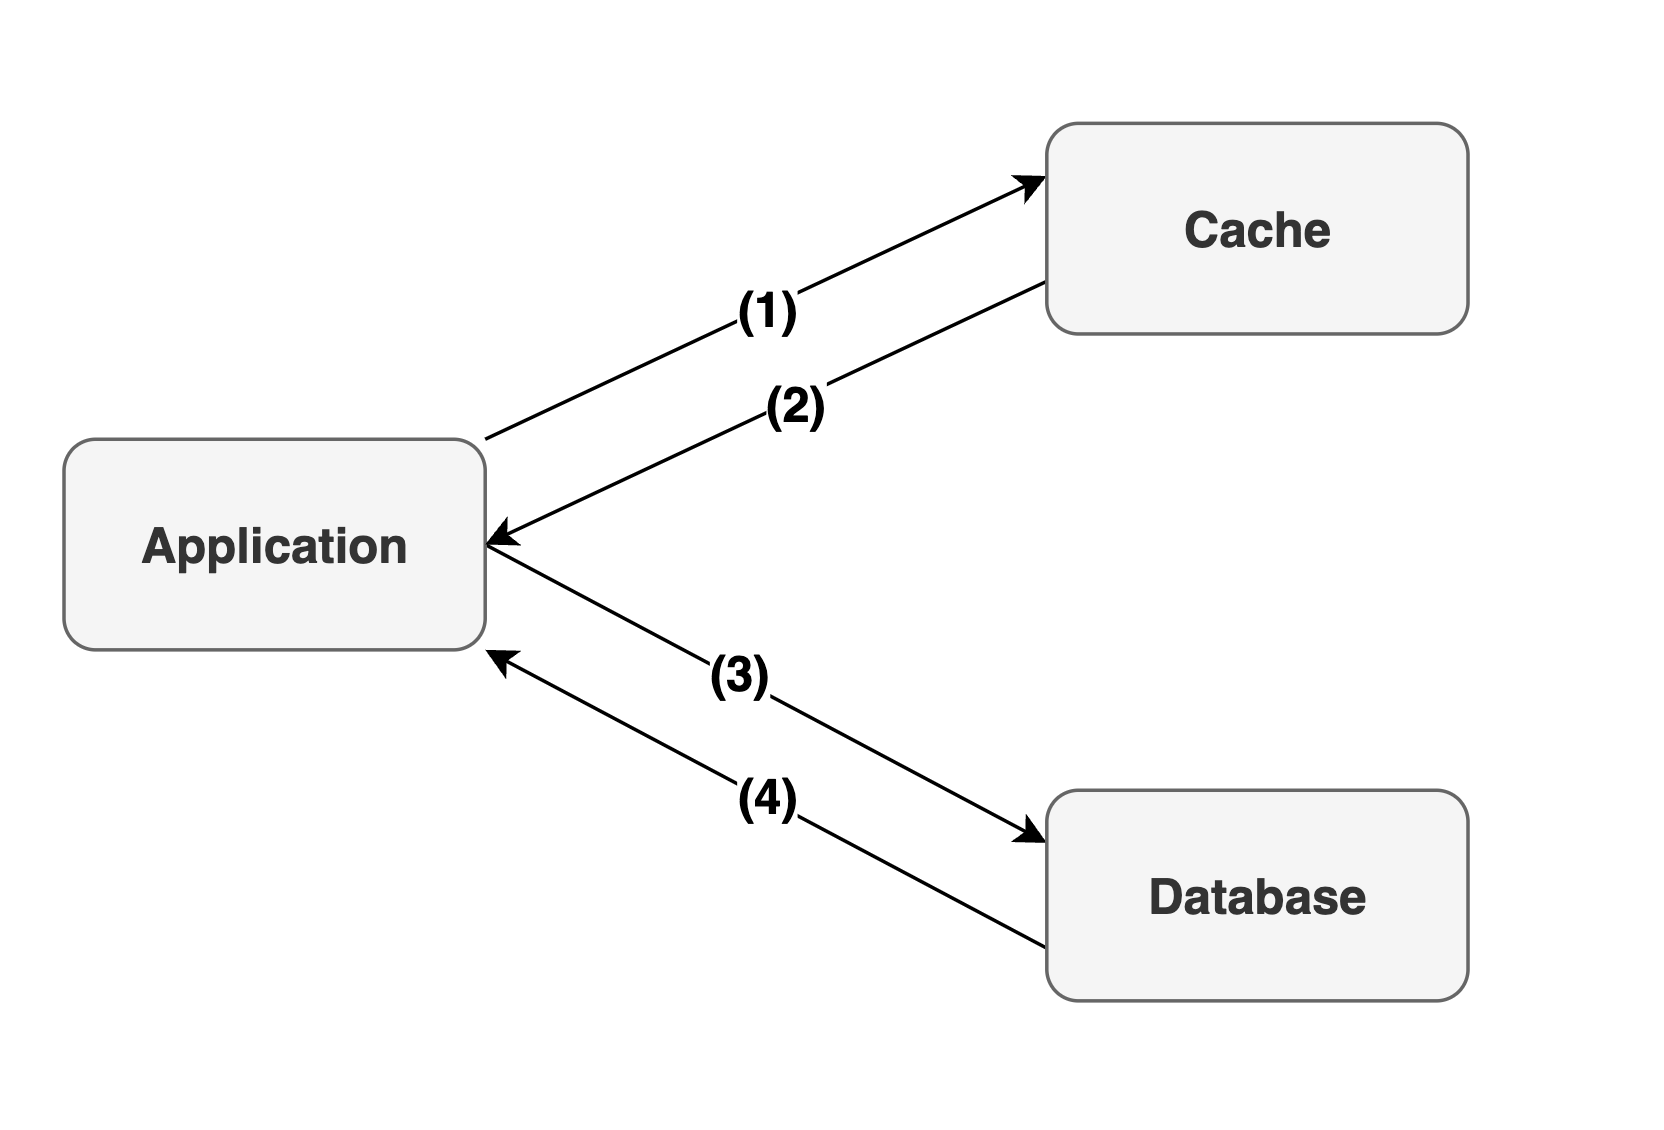
\includegraphics[width=0.8\textwidth]{Figures/caching_strat.png}
    \caption{Caching Mechanism}
\end{figure}

\section{Advanced search strategy}

Querying data that requires applying many filters (pet profiles, etc)
from the SQL database is extremely time-consuming. Note that only data
that is used repeatedly and is not too large in size can be stored
temporarily in the cache server. Therefore, applying a search strategy
to optimize querying the above type of data is necessary.

\emph{Figure 5.2} shows the steps of syncing data from the SQL database
to the Elastic-search database.

\begin{itemize}
    \item
          Whenever the application does an action on a record of the SQL
          database (create, update, delete), a new record (which includes the ID
          of the record taken the action, and the action), from now we call the
          async record, is created.
    \item
          At the end of the application process, a background job is triggered
          to query all the async records and send all the records that they
          point to onto the Elastic-search database. Therefore the data of the
          Elastic-search database is always synchronized with the SQL database.
    \item
          Note that the application only queries data from the Elastic-search
          database for tables that were defined before.
\end{itemize}

\begin{figure}[H]
    \centering
    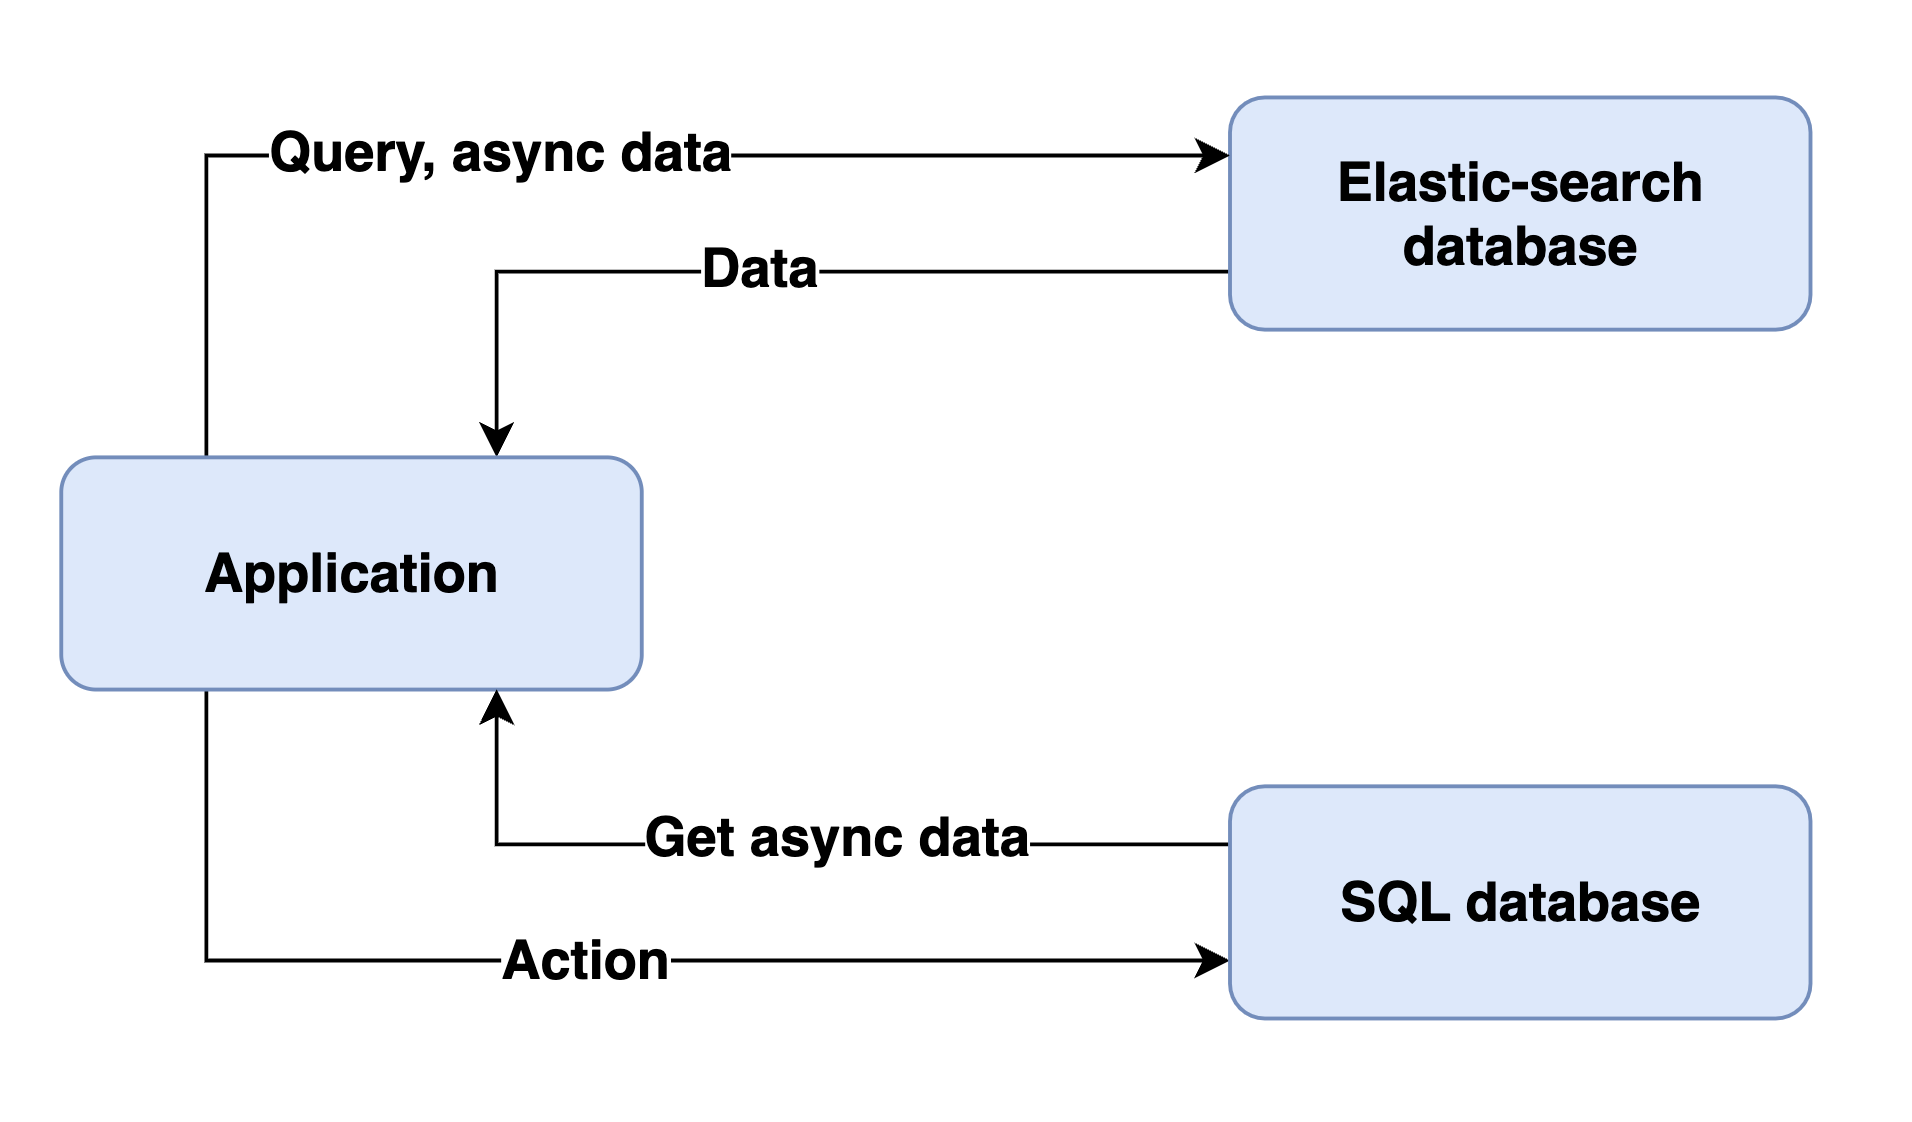
\includegraphics[width=0.8\textwidth]{Figures/search_strat.png}
    \caption{Search strategy}
\end{figure}

\section{Online payment}

In our system, we have integrated the PayPal Braintree Gateway to handle online payments securely and efficiently. Braintree is a full-stack payment platform that offers a seamless payment experience, supporting various payment methods, including credit cards, PayPal, and other digital wallets. Its robust infrastructure and comprehensive SDKs for both client and server sides make it an ideal choice for our system's payment processing needs.

\begin{figure}[H]
    \centering
    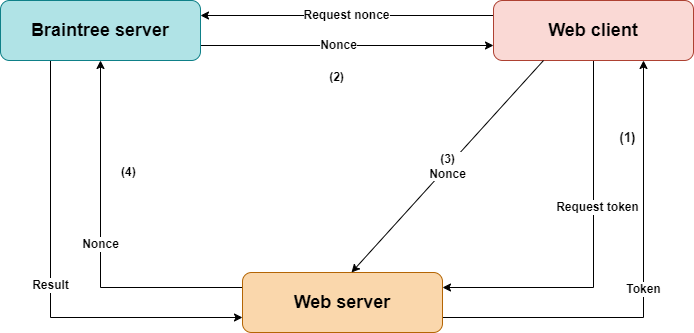
\includegraphics[width=0.7\textwidth]{Figures/payment-strat.png}
    \caption{Payment process}
\end{figure}

\emph{Figure 5.3} breaks down how the payment process is implemented:

- Step 1:
The front-end requests a client token from our server and initializes the Braintree client. This token is essential for securely communicating between the client and the Braintree server.

- Step 2:
Our server generates a client token using Braintree's tools and sends it back to the client. This token allows the front-end to securely handle customer payment information.

- Step 3:
The customer enters their payment information on the front-end. The Braintree client communicates this information to Braintree and returns a payment method nonce, a secure reference representing the payment details.

- Step 4:
The front-end sends the payment method nonce to our server. This nonce is a secure way to pass payment information without exposing sensitive data.

- Step 5:
The server receives the payment method nonce and uses Braintree's tools to process the payment. The server then communicates with Braintree to complete the transaction securely.

By utilizing PayPal Braintree Gateway, we ensure a secure and streamlined payment process, enhancing the user experience and maintaining high security standards in handling sensitive payment information.

\section{Google Login}
Our website provides users with the option to log in using their Google account, 
offering a convenient and secure authentication method. By integrating Google Sign-In, 
we simplify the login process for users and enhance the overall user experience. 

The Google Login process is illustrated in \emph{Figure 5.4}:
\begin{figure}[H]
    \centering
    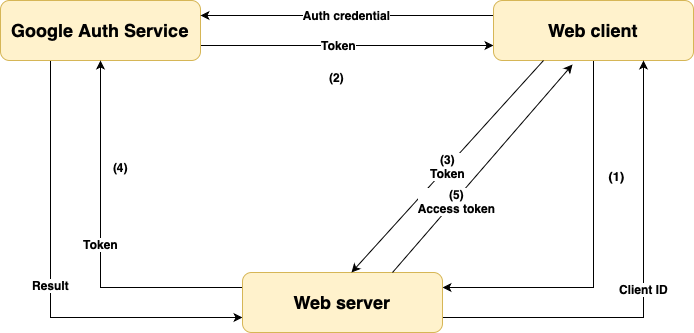
\includegraphics[width=0.7\textwidth]{Figures/Implementation/GoogleLogin.png}
    \caption{Google Login Process}
\end{figure}

The implementation steps are as follows:
\begin{itemize}
    \item Step 1: The web client obtains the client ID from the web server.
    \item Step 2: When the user clicks the Google login button, the web client displays the Google Login form. The user logs in using their Google account, and Google generates a token, which is sent back to the web client.
    \item Step 3: The web client sends the token to the web server.
    \item Step 4: The web server verifies the token with Google. If the token is valid, Google confirms this to the web server.
    \item Step 5: The web server creates an access token and sends it back to the web client. The user can now access the website using this access token.
\end{itemize}

\section{Breeds Recognition}
Breed recognition is a valuable feature for our users, who often don't know their pet's breed. To address this, we utilized ML.NET 
to train an image classification model. This advanced technology enables our platform to accurately identify a pet's breed from a photo, 
simplifying the process for users and enhancing their experience.

The first step is preparing the dataset. We have chosen the Stanford Dogs dataset\footnote{Stanford Dogs dataset: \url{https://www.kaggle.com/datasets/jessicali9530/stanford-dogs-dataset}}, which contains images of 120 dog breeds from around 
the world. This dataset, built using images and annotations from ImageNet, is ideal for the task of fine-grained image categorization. 
The challenging nature of this problem stems from the fact that certain dog breeds have nearly identical features or differ only in color and age.

For cat breed classification, we use the Cat Breeds Dataset (Cleared)\footnote{Cat Breeds Dataset (Cleared): \url{https://www.kaggle.com/datasets/denispotapov/cat-breeds-dataset-cleared}}, which contains images of 67 different cat breeds, labeled by advertisers for 
adoption. This dataset is a refined version of the original Cat Breeds Dataset from Kaggle \footnote{Stanford Dogs dataset: \url{https://www.kaggle.com/ma7555/cat-breeds-dataset}}. 
The cleared version has been meticulously cleaned to remove non-cat images, indistinguishable cat photos, duplicates, and very small images 
(height or width less than 150 pixels). This ensures that the dataset is of high quality, facilitating accurate training and performance of our 
machine learning model.

The images in the dataset are organized into separate folders for each dog breed, simplifying the model training process. This organization 
makes it more convenient to manage and feed the data into our machine learning model. Using this well-structured dataset, we can effectively 
train our image classification model with ML.NET to recognize and categorize various dog breeds accurately.

The next step involves using ML.NET Model Builder to transform our image set into an image classification model. Here's how we proceed:
\begin{enumerate}
    \item Load the Data: Import the cleaned datasets for dog and cat breeds into the ML.NET Model Builder. These datasets include images 
    categorized into folders based on their respective breeds.
    \item Set Up the Environment: Configure the Model Builder environment on our local machine, ensuring that all necessary tools and dependencies are installed.
    \item Select the Scenario: Choose the 'Image Classification' scenario in ML.NET Model Builder, which is specifically designed for tasks like breed recognition.
    \item Train the Model:
    \begin{itemize}
        \item Data Preprocessing: The Model Builder automatically preprocesses the images, resizing and normalizing them as required.
        \item Model Selection and Training: The tool selects a suitable pre-trained model and fine-tunes it using our dataset. This involves 
        splitting the data into training and validation sets to ensure the model learns effectively and generalizes well.
        \item Local Training: The model is trained on our local machine, leveraging available computational resources to iterate through 
        the dataset and optimize the classification accuracy.
    \end{itemize}
    \item Evaluate the Model: Once training is complete, the Model Builder evaluates the model's performance, 
    providing metrics such as accuracy, precision, recall, and F1 score. This helps in understanding how well 
    the model distinguishes between different breeds.
    \item Export the Model: Finally, the trained model is exported for integration into our application. 
    The Model Builder generates the necessary code and files, making it straightforward to deploy the model.
    In our case, we export the model as an API, allowing seamless integration with our platform for real-time breed recognition.
\end{enumerate}